\let\negmedspace\undefined
\let\negthickspace\undefined
\documentclass[journal]{IEEEtran}
\usepackage[a5paper, margin=10mm, onecolumn]{geometry}
%\usepackage{lmodern} % Ensure lmodern is loaded for pdflatex
\usepackage{tfrupee} % Include tfrupee package

\setlength{\headheight}{1cm} % Set the height of the header box
\setlength{\headsep}{0mm}     % Set the distance between the header box and the top of the text

\usepackage{gvv-book}
\usepackage{gvv}
\usepackage{cite}
\usepackage{amsmath,amssymb,amsfonts,amsthm}
\usepackage{algorithmic}
\usepackage{graphicx}
\usepackage{textcomp}
\usepackage{xcolor}
\usepackage{txfonts}
\usepackage{listings}
\usepackage{enumitem}
\usepackage{mathtools}
\usepackage{gensymb}
\usepackage{comment}
\usepackage[breaklinks=true]{hyperref}
\usepackage{tkz-euclide} 
\usepackage{listings}
% \usepackage{gvv}                                        
\def\inputGnumericTable{}                                 
\usepackage[latin1]{inputenc}                                
\usepackage{color}                                            
\usepackage{array}                                            
\usepackage{longtable}                                       
\usepackage{calc}                                             
\usepackage{multirow}                                         
\usepackage{hhline}                                           
\usepackage{ifthen}                                           
\usepackage{lscape}
\begin{document}

\bibliographystyle{IEEEtran}
\vspace{3cm}
\title{9.9.2.30}
\author{EE24BTECH11032 - John Bobby}
% \maketitle
% \newpage
{\let\newpage\relax\maketitle}

\renewcommand{\thefigure}{\theenumi}
\renewcommand{\thetable}{\theenumi}
\setlength{\intextsep}{10pt} % Space between text and floats


\numberwithin{equation}{enumi}
\numberwithin{figure}{enumi}
\renewcommand{\thetable}{\theenumi}


\textbf{Question:}Calculate the area under the curve $y=2\sqrt{x}$ included with the lines $x=1$ and $x=0$.\\
\begin{table}[h!]    
  \centering
  \begin{tabular}[12pt]{ |c| c|}
    \hline
        \textbf{Variable}  & \textbf{Description}\\
    \hline
        $a,b$ &  Variables inside the coordinates\\
    \hline 
        $\vec{P}\brak{9a-2,-b}$ & coordinates of point $P$\\
    \hline
	$\vec{A}\brak{3a+1.-3}$ & coordinates of point $A$\\
    \hline
	$\vec{B}\brak{8a,5}$ & coordinates of point $B$\\
    \hline
	$k$ & ratio in which P divides $\vec{AB}$\\
    \hline 
\end{tabular}

  \caption{Input Parameters}
  \label{tab9.9.2.30}
\end{table}


\solution For a line $\vec{x}=\vec{h}+k\vec{m}$,the intersection of the line with a conic with parameters $\vec{V},\vec{u},\vec{h},\vec{m}$ and h is given by $\vec{x}=\vec{h}+k_i\vec{m}$\\
 $L_1:x=0$\\
$L_2:x=1$\\
\begin{align}
	k_i &= \frac{1}{\vec{m}^\top \vec{Vm}}\brak{-\vec{m}^\top \brak{\vec{Vh}+\vec{u}}+ \sqrt{\sbrak{\vec{m}^\top \brak{\vec{Vh}+\vec{u}}}^2-g\brak{\vec{h}}\brak{\vec{m}^\top 	    \vec{Vm}}}}
\end{align}
on solving for $L_1$ and $L_2$
\begin{align}
	k_1 &=0,k_2=2\\
	\vec{A}&=\vec{h_1}+k_1\vec{m_1}=\myvec{0\\0}+0\myvec{0\\1}=\myvec{0\\0}\\
	\vec{B}&=\vec{h_2}+k_2\vec{m_2}=\myvec{1\\0}+2\myvec{0\\1}=\myvec{1\\2}
\end{align}
Thus the area under the curve included with the lines $x=1$ and $x=0$ is given by
\begin{align}
	\int_{0}^{1} 2\sqrt{x} \,dx &=\brak{\frac{4}{3}x^\frac{3}{2}}\limits_{0}^{1} \ =\frac{4}{3}
\end{align}
\begin{figure}[h!]
                \centering
               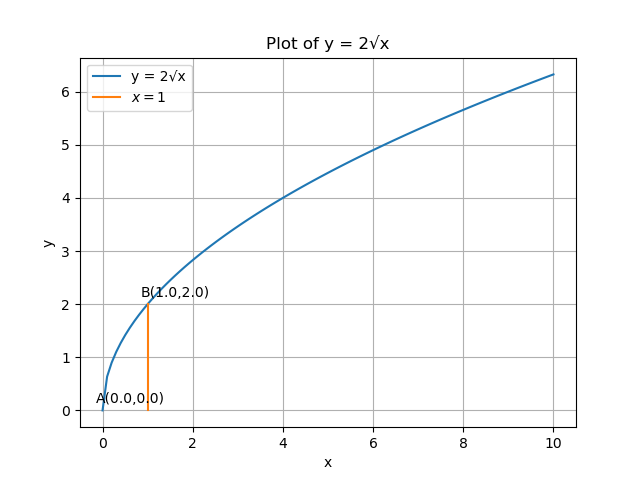
\includegraphics[width=0.7\linewidth]{Figs/Fig1.png}
			\caption{Plot of Parabola}
               \label{stemplot}
               \end{figure}




\end{document}
